%%%%%%%%%%%%%%%%%%%%%%%%%%%%%%%%%%%%%%%%%%%%%%%%%%%%%%%%%%%%%%%%%%%%%%%%%%
%%%%%                         CHAPITRE 4                            %%%%%%
%%%%%%%%%%%%%%%%%%%%%%%%%%%%%%%%%%%%%%%%%%%%%%%%%%%%%%%%%%%%%%%%%%%%%%%%%%

\lhead[\fancyplain{}{\leftmark}]%Pour les pages paires \bfseries
      {\fancyplain{}{}} %Pour les pages impaires
\chead[\fancyplain{}{}]%
      {\fancyplain{}{}}
\rhead[\fancyplain{}{}]%Pour les pages paires 
      {\fancyplain{}{\rightmark}}%Pour les pages impaires \bfseries
\lfoot[\fancyplain{}{}]%
      {\fancyplain{}{}}
\cfoot[\fancyplain{}{\thepage}]%\bfseries
      {\fancyplain{}{\thepage}} %\bfseries
\rfoot[\fancyplain{}{}]%
     {\fancyplain{}{\scriptsize}}


%%%%%%%%%%%%%%%%%%%%%%%%%%%%%%%%%%%%%%%%%%%%%%%%%%%%%%%%%%%%%%%%%%%%%%%%%%
%%%%%                      Start part here                          %%%%%%
%%%%%%%%%%%%%%%%%%%%%%%%%%%%%%%%%%%%%%%%%%%%%%%%%%%%%%%%%%%%%%%%%%%%%%%%%%

\chapter{Robustness assessment}
\label{ch:4}

%==============================================================================	Résumé du chapitre

\begin{center}
\rule{0.7\linewidth}{.5pt}
\begin{minipage}{0.7\linewidth}
\smallskip

\textit{a\newline \newline
This chapter is adapted from the article published in the Sensors: "Pose2Sim: An End-to-End Workflow for 3D Markerless Sports Kinematics—Part 1: Robustness" \cite{Pagnon2021}.
}

%\smallskip
\end{minipage}
\smallskip
\rule{0.7\linewidth}{.5pt}
\end{center}

\minitoc
\newpage


\section{Introduction}
\subsection{Robustness definition}

According to the review of \cite{Desmarais2021}, the performance of a method can be ranked regarding its accuracy, speed, or robustness. Accuracy is mostly assessed with MPJPE (Mean Per Joint Position Error); speed is evaluated either regarding computing complexity, or framerate when possible; and robustness is gauged through differences in the results while changing the system parameters only. \cite{Desmarais2021} points out that authors usually only consider accuracy, sometimes speed, but rarely robustness. However, robustness is of paramount importance in the context of sports, especially "in the wild". This chapter will focus on robustness, the next one on \nameref{ch:5}, and we will not focus on speed in this thesis (although chapter 3.4.5 broaches \hyperref[subsec:realtime]{Real time considerations}).

\cite{Moeslund2001} proposed to express robustness as the number of constraints on the subject or on the environment required for a motion capture system to be operational. Some of the assumptions they proposed have already been universally overcome by deep-learning-based methods. For example, no markers are involved anymore, the subject can wear their usual clothes (including loose pants or dresses \cite{Viswakumar2019}), and the background does not need to be static or uniform. Some other items remain an open problem.

For instance, most 3D methods assume that only one person lies in the camera field of view. This is a strong assumption, especially outdoors where people and athletes pass by and an operator is often present. Although it is starting to be addressed, standard solutions are yet to be determined \cite{Slembrouck2020,Bridgeman2019, Chu2021, Dong2019}. 

Other open questions lie in the environment, much less controlled in a sports context than in a lab, which can result in bad image qualities. \cite{Viswakumar2019} experienced that OpenPose is very robust to extreme lightning conditions. However, research has shown that pose estimations models are more robust to noise or brightness changes, while less robust to motion or to defocus blur \cite{Wang2021b}. And yet, in sports, the movement is not usually slow, continuous, nor limited to the sagittal plane.

Occlusions are, for the most part, solved by using a network of calibrated cameras. Since triangulation is computed using a least square method, a large amount of cameras will also blunt imprecision on the 2D joint estimations. \cite{Bala2020} showed that once correctly trained for 3D macaque pose estimation, eight cameras were enough to correctly infer 80\% of the 13 considered keypoints, while four cameras decreased the performance to about 50\%. However, a correct estimation of extremities such as feet and hands required more than eight cameras.

Camera calibration can be challenging outside, due to large volume spaces, bright light, and contrasting shades. As a consequence, it is close to impossible with the classic approach based on predefined objects with markers. Moreover, simple calibration with a checkerboard may cause errors on intrinsic and extrinsic camera parameters estimation \cite{Sun2005}. A calibration is generally considered acceptable if the average residuals of each camera (i.e., the root mean square error of the reprojection of the 3D reconstructed coordinates on the 2D image plane) is below 1 pixel. In metric terms, the markers-based Qualisys Track Manager software recommends redoing a calibration when the average residuals exceed 3 millimeters \cite{QTM2018}. The pinhole camera model gives an equivalence between pixel values on the image plane, and metric values on the object plane at the center of the scene, as demonstrated by Figure~\ref{fig_pixmeterscorrespondance} and Equation~\ref{eqn:errobjimg}. See Chapter 2.2.1 on \nameref{subsec:Pinhole model} or \cite{Dawson-Howe1994} for in-depth explanations.

\begin{figure}[!ht]
	\centering
	\def\svgwidth{1\columnwidth}
	\fontsize{10pt}{10pt}\selectfont
	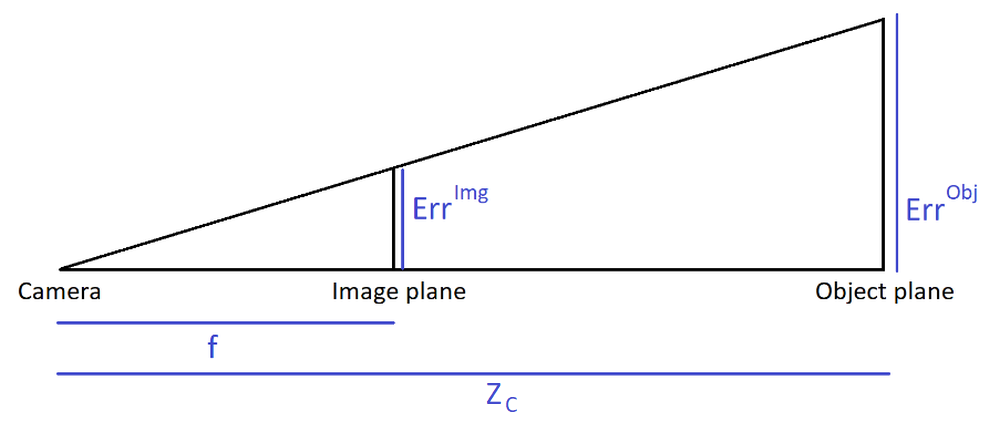
\includegraphics[width=\linewidth]{"../Chap4/Figures/Fig_PixelMeterCorrespondance.png"}
	\caption{The pinhole camera model permits a correspondence between image coordinates and object coordinates. f: focal distance, D: object to camera distance, $Err^{Img}$: error on image plane, $Err^{Obj}$: error on object plane. f and $Err^{Img}$ are usually expressed in pixels, while D and $Err^{Obj}$ are expressed in meters.}
	\label{fig_pixmeterscorrespondance}
\end{figure}

\begin{equation}
      Err^{Img} = \frac{f \times Err^{Obj}}{D} 
      \label{eqn:errobjimg}
\end{equation}


\subsection{Assessing robustness}

Before assessing the robustness of the workflow on walking, running, and cycling sequences, the relevance of the computed 3D full-body angles needs to be estimated. This will be done by comparing our angle results to those of a normative walking database. Further concurrent validation of the accuracy will be determined in the next chapter on \nameref{ch:5}. Repeatability will be evaluated by comparing movement cycles to each other, within each task and each capture condition. 

Robustness itself will be assessed through all three types of movements, in accordance with the open problems previously described:
\begin{enumerate}[itemsep=0em, topsep=0em, leftmargin=*]
      \item In addition to the person of interest, some people will be present in the background. 
      \item Image quality will be altered, by simulating a dark scene captured with defocused cameras objectives.
      \item Occlusions will become more challenging as we decrease the number of cameras. Moreover, cycling sequences will lead to more occlusions than walking or running ones.
      \item Calibration errors will be introduced by corrupting the calibration files.
\end{enumerate}

The underlying idea presented in this article is to verify whether modifying external environment parameters significantly impacts variability in joint angle estimation.


\section{Methods}
\subsection{Experimental setup}

To guarantee a tight control of the environment parameters, we captured our data in a dedicated studio platform, which is able to create realistic virtual views similar to outdoor video. This platform was a \(10 m \times 10 m \times 5.6 m\) green room equipped with 68 cameras recording at 30 fps in 4 Mpixels resolution, for a practical acquisition space of about \(5 m  \times 5 m  \times 3 m\). The system computes 3D textured meshes by convex visual hull reconstruction (See Laurentini [66]). The meshes were inserted in a virtual environment composed of an environment texture map captured from a BMX racetrack, and a custom-made virtual floor. It should be noted that three people were present in the background, which introduced a realistic artefact of multiple subjects.

We developed a script for the Autodesk Maya (similarly, we plan to release the code as open source with Part 2 of this series of articles) software that allows us to render the textured mesh files, as well as to virtually set any cameras with specific properties (position, orientation, resolution, focal length, distortion, pixel size, binning factor). Views seen through virtual cameras can be saved as video files and visualized into a global 3D environment (Figure 3). The generated video files were used as input to the 3D kinematics pipeline.

Sensors 21 06530 g003 550Figure 3. The camera toolbox developed for Autodesk Maya, which lets one set up virtual cameras, save their parameters in a calibration file, and film realistic looking synthetic videos. Here, we set up 8 video cameras, regularly distributed 8 m away from the subject.

For the purpose of this study, we created 8 virtual video cameras (resolution \(1280 \times 768 px\), focal length 9 mm, no distortion, pixel size 5.54 µm, and no binning). Binning refers to the process of grouping pixels in order to increase sensitivity to light at the expense of decreasing resolution. Cameras were regularly distributed 8 m away from the center of the captured volume, at a height of 1 m, so that the whole body could be detected for a maximum of cycles. We then rendered the scene as video files from our virtual cameras and saved the exact calibration parameters. We applied a \(3 \times 3) pixel Gaussian blur afterwards to reduce sharp edges of the virtual scene compositing (Figure 4). This resulting image quality is considered as “standard”.

Sensors 21 06530 g004 550Figure 4. To smooth out sharp edges due to compositing, we applied a 3 × 3 pixel Gaussian blur to the videos filmed from our virtual scene.


\subsection{Participant and protocol}
\blindtext

\subsection{Challenging robustness}
\blindtext

\subsection{Statistical analysis}
\blindtext


\section{Results}
\subsection{Data collection and 2D pose estimation}
\blindtext

\subsection{Pose2Sim tracking, triangulation, and filtering}
\blindtext

\subsection{Relevance, repeatability and robustness of angles Results}
\blindtext


\section{Discussion}
\subsection{Pose2Sim}
\blindtext

\subsection{Relevance, repeatability and robustness}
\blindtext

\subsection{Limits and perspectives}
\blindtext
